\section{\label{secResults}Results}

\subsection{\label{ptspectra}Transverse momentum distributions} 

The transverse momentum distributions measured at midrapidity for the 
event classes defined in Tab.~\ref{tab:OverviewEventClasses} are shown in Fig.~\ref{fig:UIDspectra}
for unidentified charged particles ($|\eta| < 0.5$) and Fig.~\ref{fig:spectra} for  \pipm, \kapm, \kzero, \kstar, \p, \pbar, $\phi$, 
$\lmb$, $\almb$, \X, \Ix, \Om\ and \Mo ($|y| < 0.5$). In the particular case of the $\phi$, \kstar\ and \Om\ measurements, some event classes were merged to allow for sufficient statistics. Particle and antiparticle as well as charged and neutral kaon production rates are compatible within uncertainties.

\begin{figure*}[htb!]
  \begin{flushleft}
    %\center{\includegraphics[width=0.49\textwidth]{figures/V0M05errorsAllSpectra.pdf}
    \center{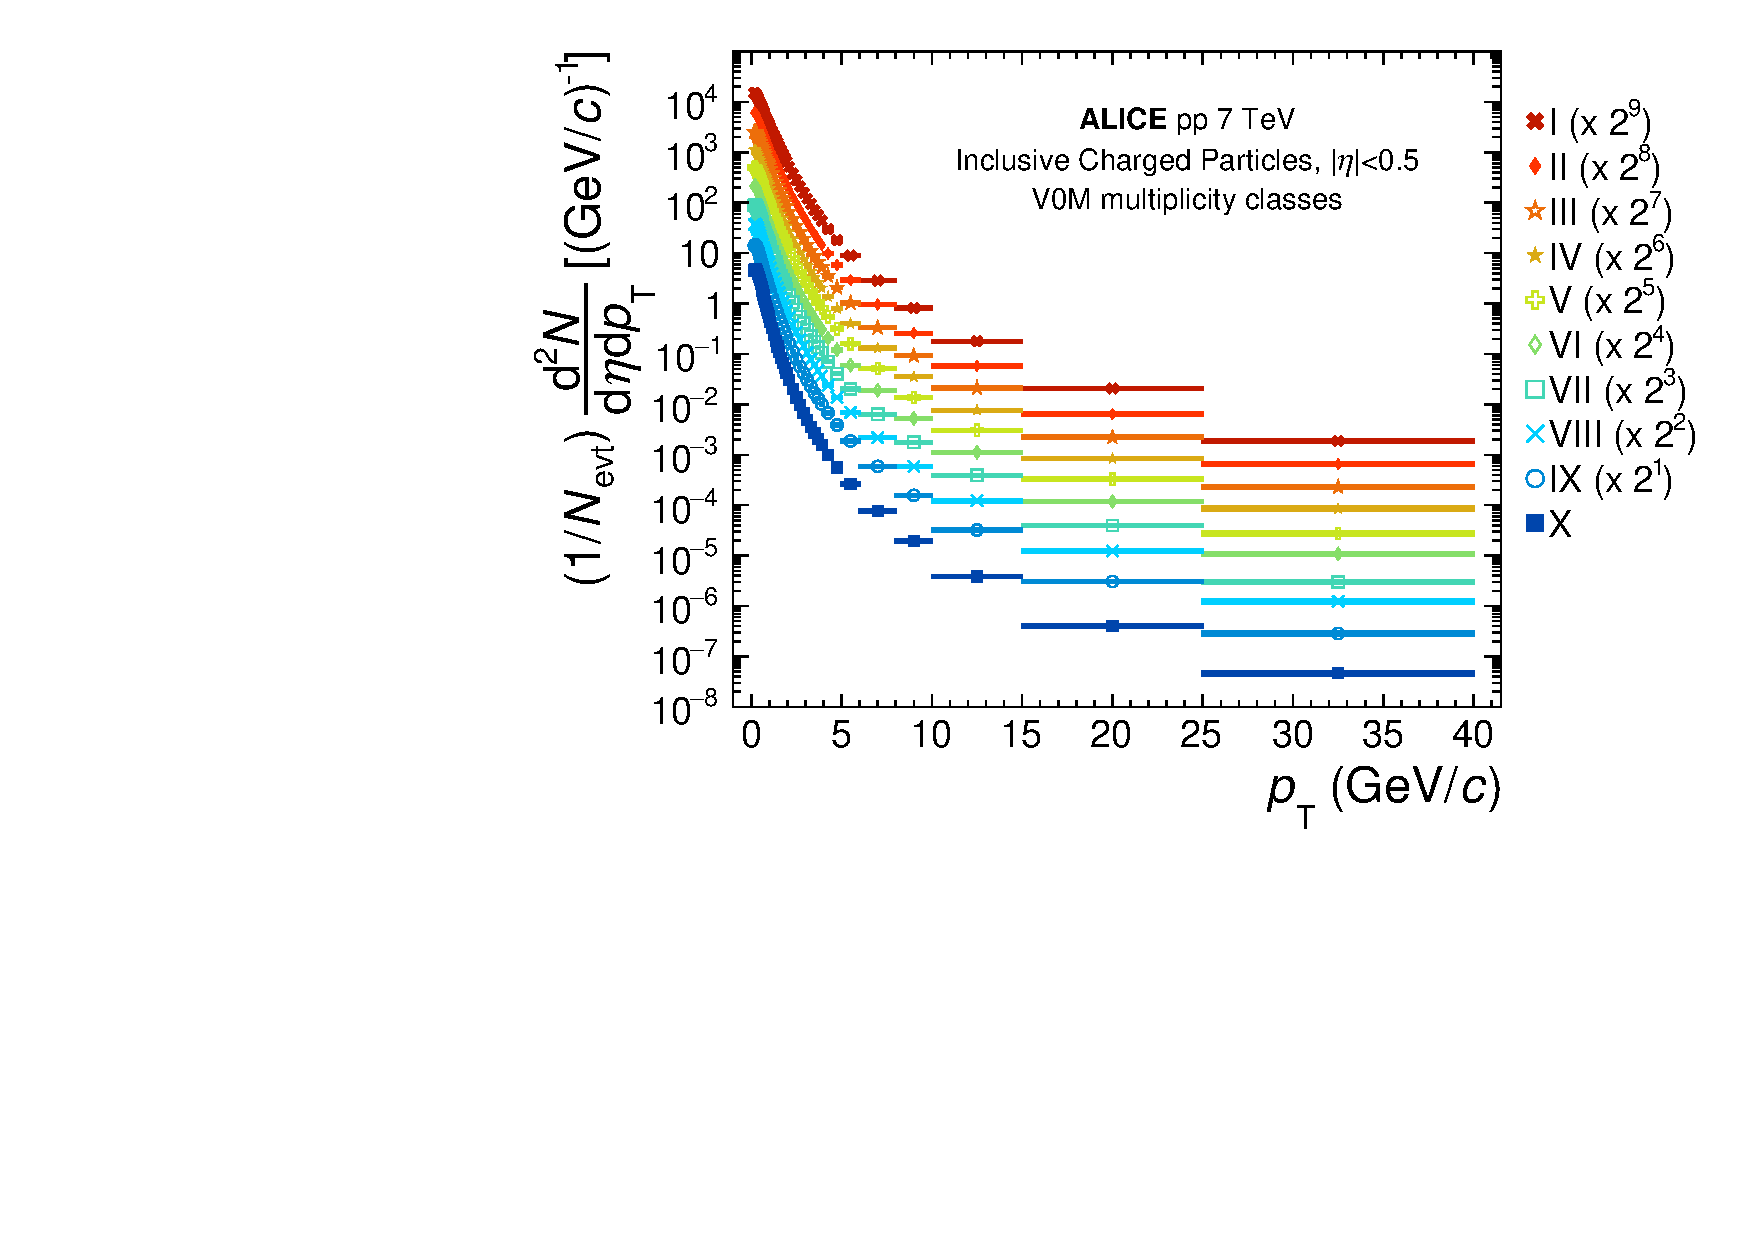
\includegraphics[width=0.75\textwidth]{figures/Spectra_V0M_summedCharges_1_LS_RM.pdf}
    %\includegraphics[width=0.435\textwidth]{figures/V0M05errorsAllLogxyUncorRatioOnly.png}
    }
    \end{flushleft}
    \caption{Transverse momentum spectra of the sum of positively and negatively charged particles in different V0M event multiplicity classes.
} 
    \label{fig:UIDspectra}
\end{figure*}  

\begin{figure*}[htb!]
%  \begin{flushleft}
    \center{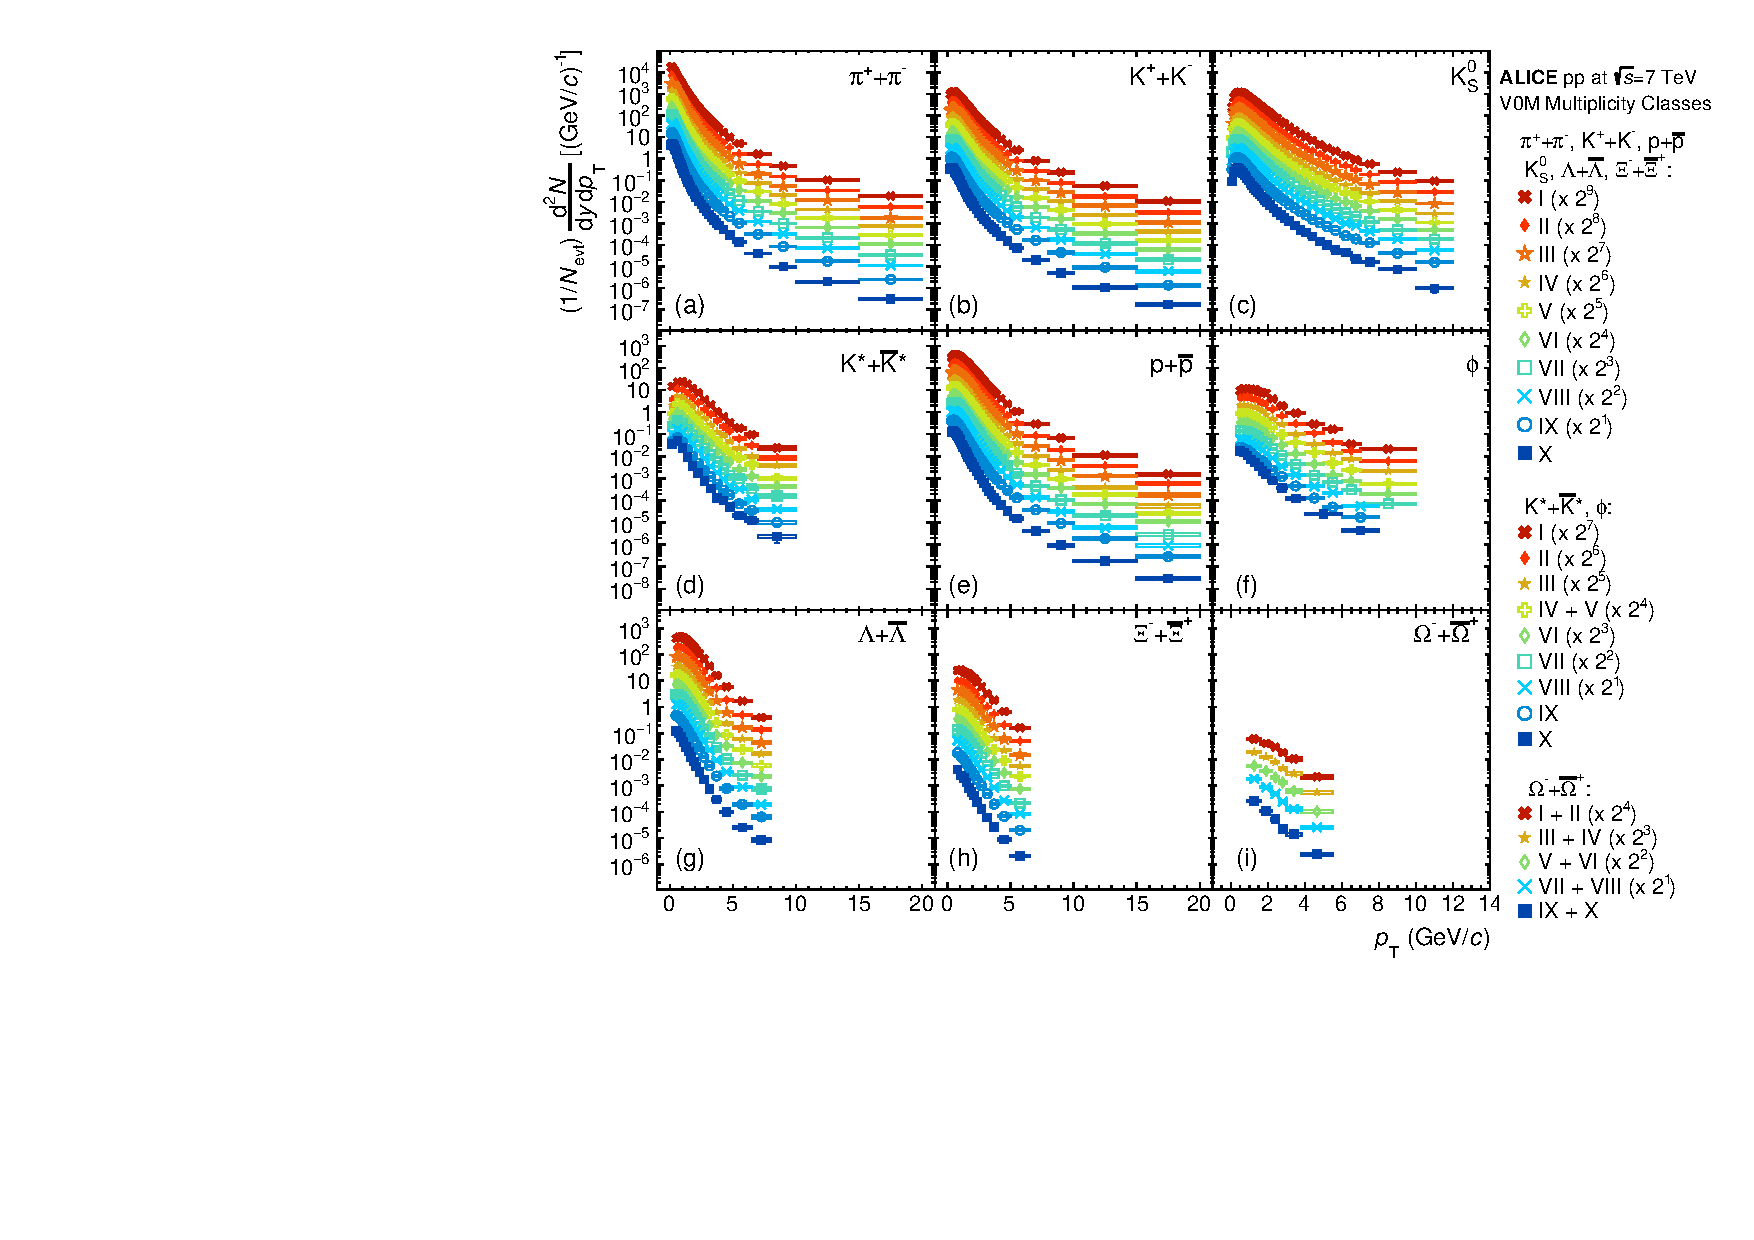
\includegraphics[width=\textwidth]{figures/Spectra_V0M_summedCharges_LS_RM.pdf}}
%    \end{flushleft}
    \caption{Transverse momentum spectra of (a) \pipm, (b) \kapm, (c) \kzero, (d) \kstar, (e) \p+\pbar, (f) $\phi$, 
(g) $\lmb$+$\almb$, (h) \X+\Ix and (i) \Om+\Mo. Top to bottom: high to low multiplicity; data are scaled by $2^{n}$ factors for better visibility. }
    \label{fig:spectra}
\end{figure*}  

Transverse momentum spectra are observed to become harder with increasing charged-particle multiplicity, with absolute changes in the spectrum shapes being more pronounced for particles with larger mass. The evolution of the \pt\ distributions with respect to the spectra in the INEL$>$0 event class for the various particle species is shown in Fig.~\ref{fig:spectramodification} and is observed to be identical for the two \pipm\ and \kapm\ mesons as well as for the \p, \lmb, \X\ baryons and their corresponding anti-particles. The spectra modification of $\phi$ and \kstar\ resonances follows the trend observed for baryons at \pt\ $<$ 2 \gevc\, while for larger momenta the modification is similar to the one observed for other mesons. Given that these mesonic resonances have a significantly higher mass than that of \pipm\ and \kapm, this suggests that the spectra evolution with multiplicity is driven by the hadronic mass at low \pt\ and by the number of constituent quarks at higher \pt. It is also interesting to note that such behavior 
is not unique to high multiplicity, but is present even for the lowest multiplicity class, where mass-dependent 
mechanisms such as radial flow are not expected to play a significant role. 

\begin{figure*}[htb!]
%  \begin{flushleft}
\center{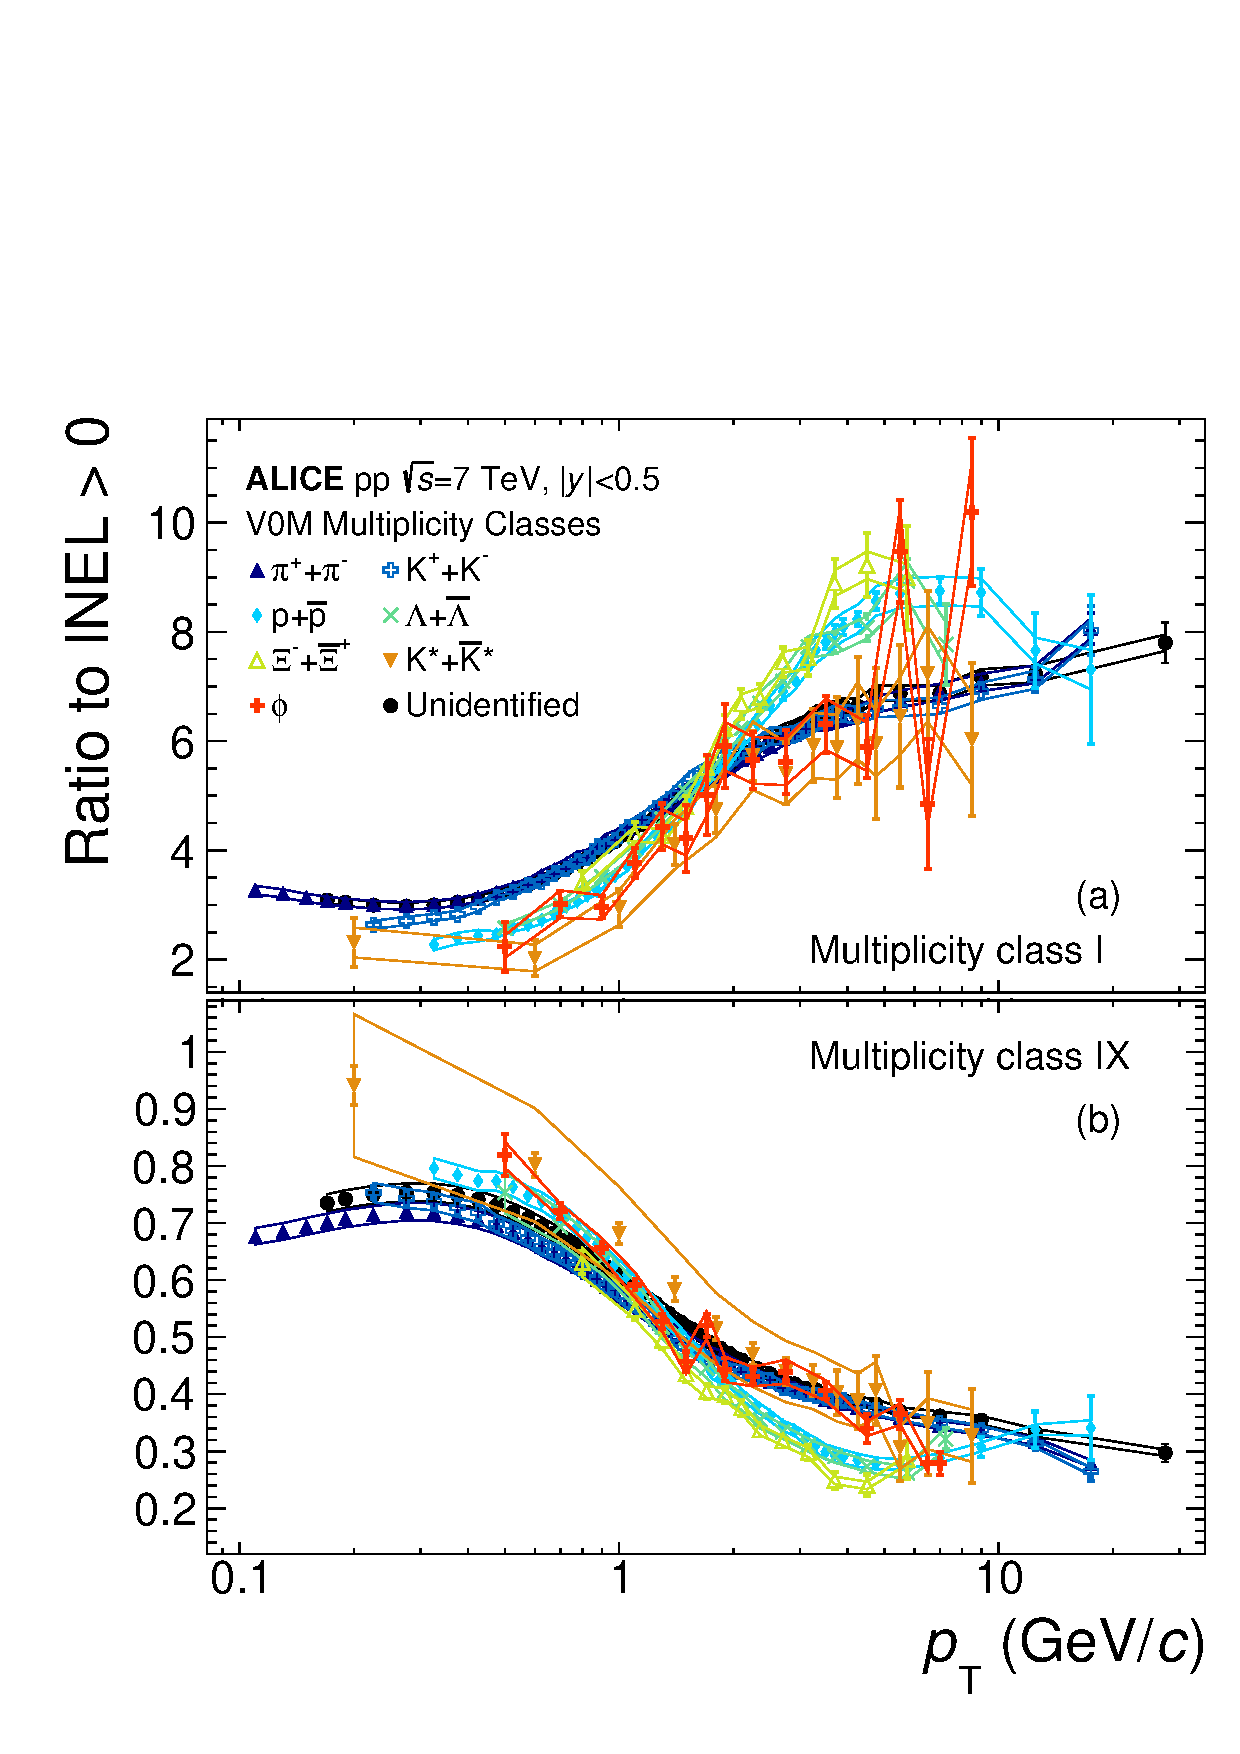
\includegraphics[width=0.8\textwidth]{figures/Results_SpectraRatioToMinBias_LogX.pdf}}
%    \end{flushleft}
    \caption{Unidentified and identified particle spectra modification in (a) high-multiplicity and (b) low-multiplicity event classes. 
    Statistical uncertainties are shown as errors bars and systematic uncertainties that are uncorrelated across multiplicities are shown as boxes. Other 
    uncertainties are disregarded as they cancel in the ratio.}
    \label{fig:spectramodification}
\end{figure*}  

A comparison of the multiplicity dependence of the transverse momentum distributions can be performed by studying the ratios \p/$\phi$~=~(p + \pbar)/$\phi$, \kpi~=~(\kap + \kam)/(\pip + \pim),  \ppi~=~(p + \pbar)/(\pip +
\pim) and  \lmb/\kzero\ as a function of
\pt, as shown in Fig.~\ref{fig:RatiosVsPt} for the lowest and highest multiplicity classes in this work. 
Results are compared with measurements in \pPb\ collisions at \fivenn~\cite{Abelev:2013haa, Adam:2015vsf, 2016720} as well as in \PbPb\ at 
\twosevensixnn~\cite{Abelev:2013xaa,2014196}. 
The \p/$\phi$ ratio is observed to decrease with \pt\ in \pp\ and 
low-multiplicity \pPb\ collisions but is seen to become progressively flatter for high-multiplicity \pPb\ and \PbPb\
collisions. Given the similar mass of the particles involved in this ratio, it is possible that this flattening is  
a signature of significant radial flow in the larger systems. 
Furthermore, the baryon-to-meson ratios  \ppi\ and \lmb/\kzero\ exhibit a characteristic depletion at \pt~$\sim0.7$~\gevc\ and an enhancement at intermediate \pt\ ($\sim3$~\gevc), which is qualitatively similar to that observed in \pPb\ and \PbPb\ collisions. Finally, the \kpi\ ratio is observed to be relatively
multiplicity-independent, except for central \PbPb\ collisions, where a weak depletion (enhancement) at
low (intermediate) \pt\ is visible. 

While the observed changes in these particle ratios are quantitatively different 
in the various collision systems, it is worth noting that the final state charged particle multiplicities also cover 
very distinct ranges. If considered as a function of \dNdeta, the ratios measured in specific low-, mid- and high-\pt\ intervals shown in Fig.~\ref{fig:RatiosVsNch} are seen to depend on multiplicity in a remarkably similar manner for all collision systems, despite differences in energy and collision geometry. 


\begin{figure*}[tp!]
  \begin{flushleft}
    \center{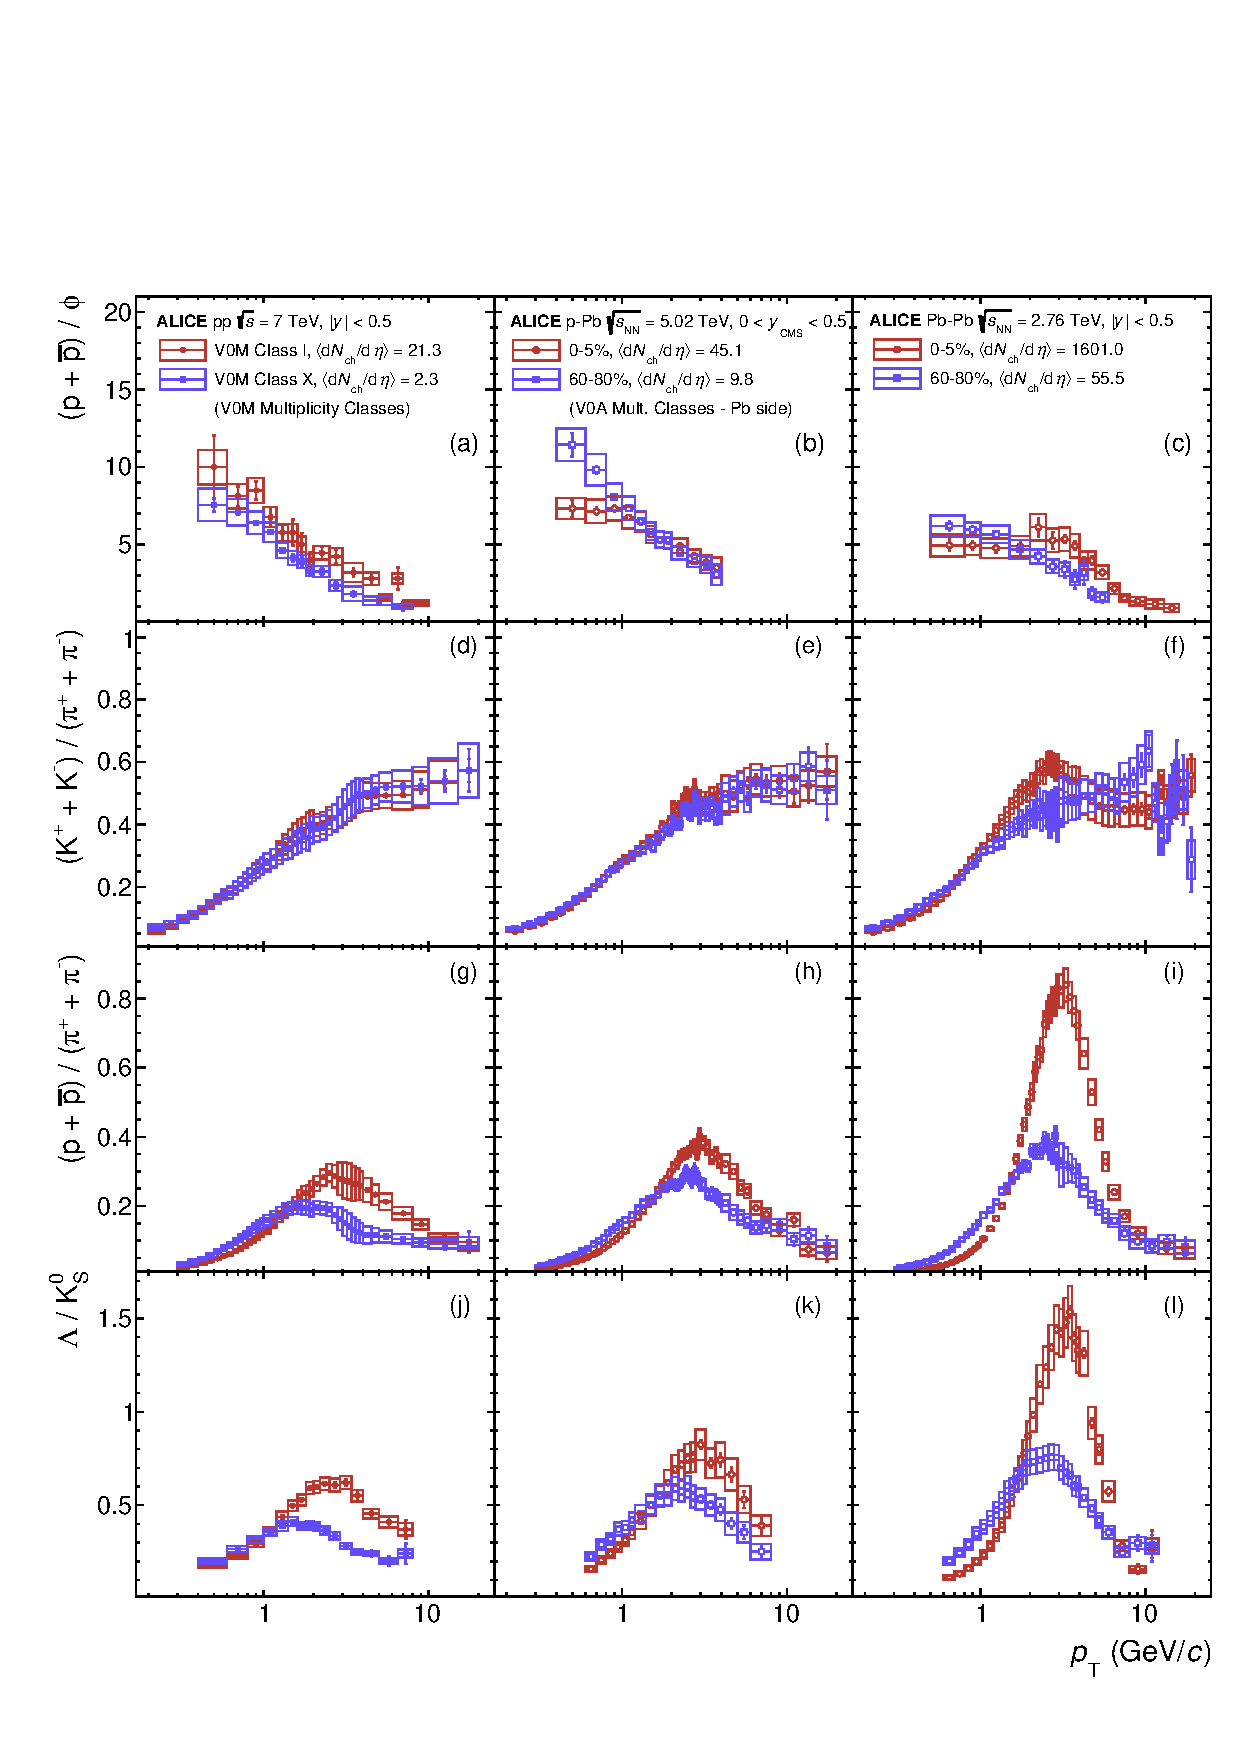
\includegraphics[width=0.99\textwidth]{figures/Results_SpectraRatio_AllSystems.pdf}}

    \end{flushleft}
    \caption{Transverse momentum dependence of (a, b, c) \p/$\phi$~=~(p + \pbar)/$\phi$, (d, e, f) \kpi~=~(\kap + \kam)/(\pip + \pim),  (g, h, i) \ppi~=~(p + \pbar)/(\pip +
\pim) and (j, k, l) \lmb/\kzero\ (from top to bottom row) yield ratios in (a, d, g, j) pp, (b, e, h, k) p-Pb and (c, f, i, l) Pb-Pb collisions for high- and 
    low-multiplicity classes, respectively. Cancellation of common systematic uncertainties in the numerator and denominator was carried
    out only for the \lmb/\kzero, as in other cases the cancellation is non-trivial because of the use of various combined identification techniques or, in the case of resonances, of significantly different analysis strategy. Reference p-Pb and Pb-Pb data from \cite{Abelev:2013haa, Adam:2015vsf, 2016720, Abelev:2013xaa,2014196}.}
    \label{fig:RatiosVsPt}
\end{figure*}  

\begin{figure*}[tp!]
  \begin{flushleft}
    \center{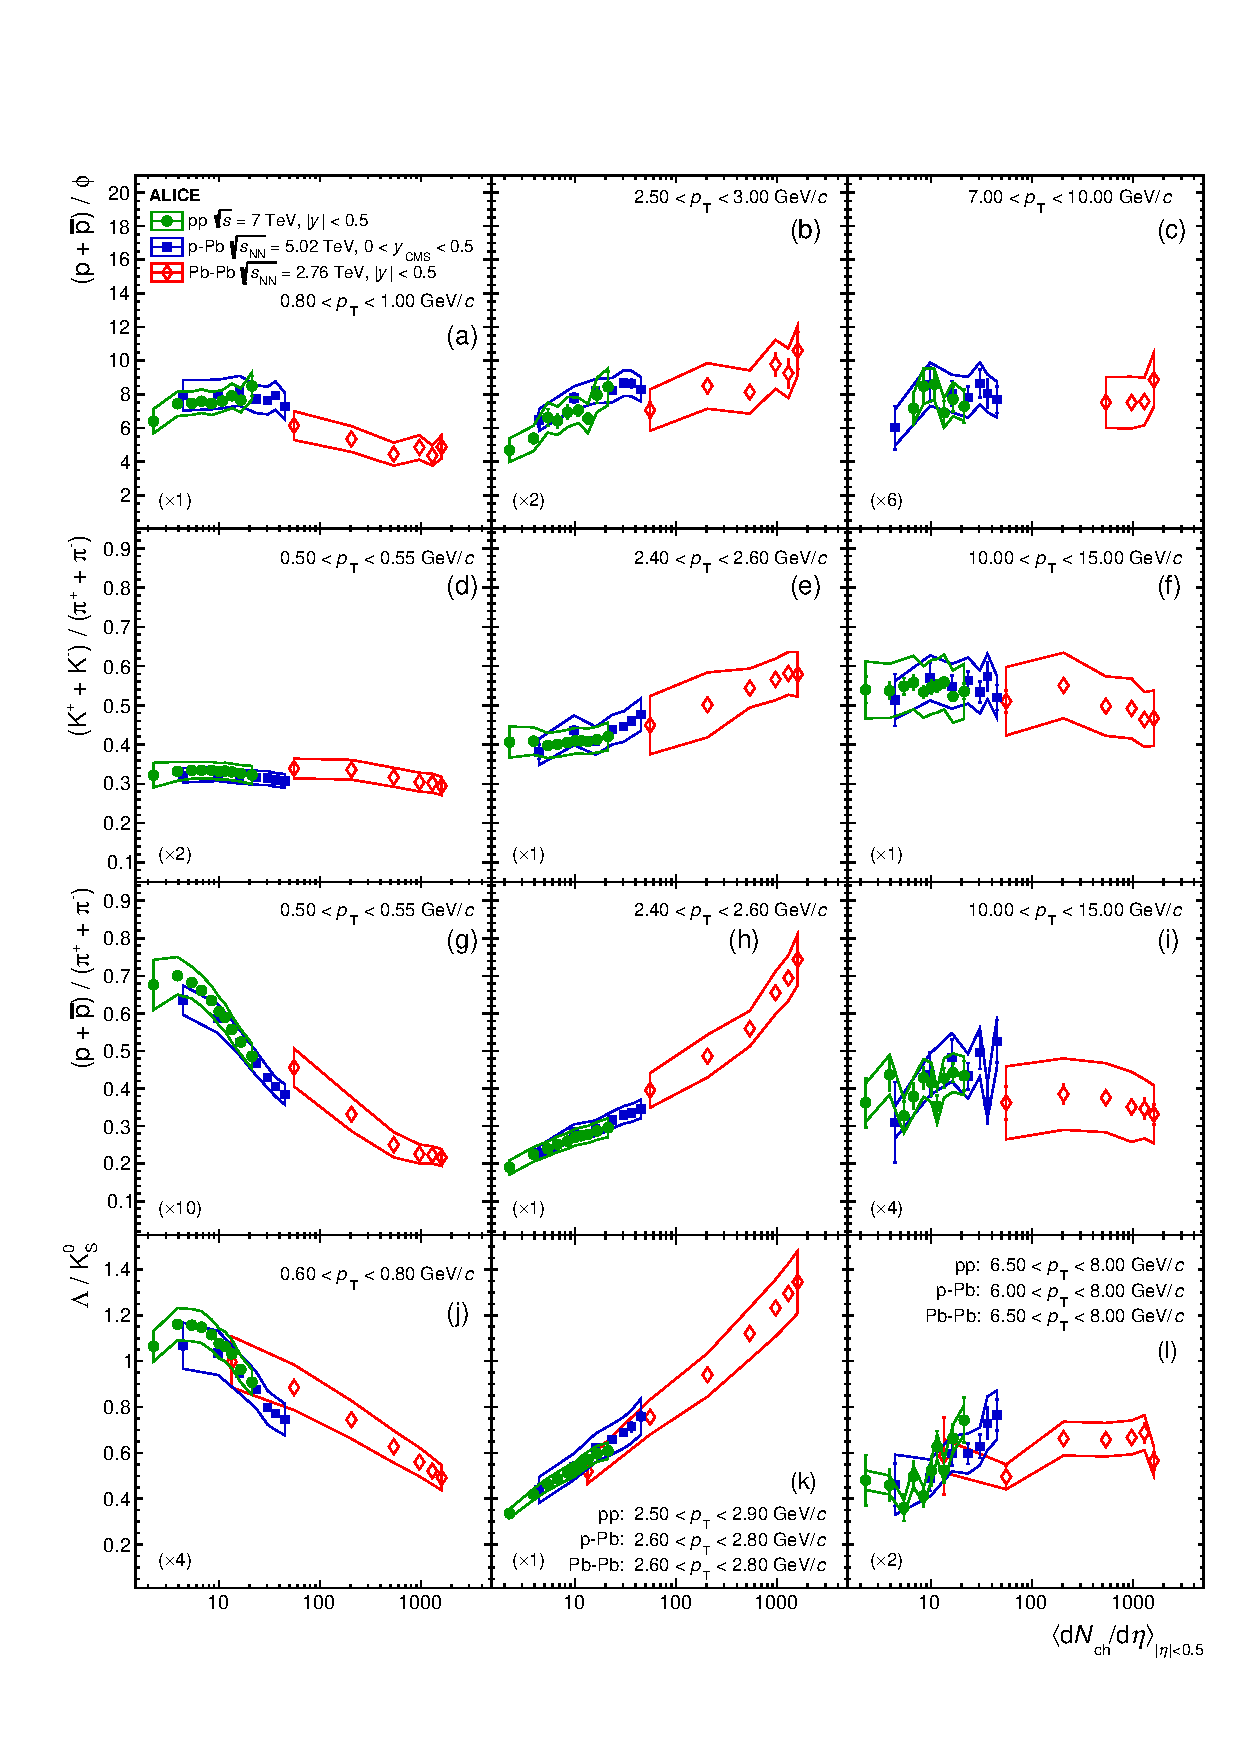
\includegraphics[width=0.99\textwidth]{figures/Results_SpectraRatioVsMult_AllSystems_withProtonOverPhi.pdf}}
    \end{flushleft}
    \caption{Transverse momentum dependence of (a, b, c) \p/$\phi$~=~(p + \pbar)/$\phi$, (d, e, f) \kpi~=~(\kap + \kam)/(\pip + \pim),  (g, h, i) \ppi~=~(p + \pbar)/(\pip +
\pim) and (j, k, l) \lmb/\kzero\ yield ratios in (a, d, g, j) low-, (b, e, h, k) mid- and (c, f, i, l) high-\pt\ intervals 
in pp, p-Pb and Pb-Pb collisions as a function of \avdNdeta. Reference p-Pb and Pb-Pb data from \cite{Abelev:2013haa, Adam:2015vsf, 2016720, Abelev:2013xaa,2014196}.} 
    \label{fig:RatiosVsNch}
\end{figure*}  
\clearpage

\subsection{\label{integrated}Integrated yields and average momenta} 

The \pt-integrated yields d$N$/d$y$ and mean transverse momenta \avpT\ have been calculated using data in the measured momentum range
 and a L\'{e}vy-Tsallis parametrization to extrapolate the spectra down to zero \pt, similarly to what 
was done in previous studies~\cite{Adam:2015qaa, Abelev2012309, Abelev:2012hy}. Several functional forms, such as
Boltzmann, \mt-exponential, \pt-exponential, Fermi-Dirac and Bose-Einstein functions, were used
to estimate the systematic uncertainties associated to this procedure. For those functions that are unable
to describe the \pt\ distributions in the full measured range, the fitting was restricted only to low-\pt. The uncertainty on \dNdy\ and \meanpt\ associated to this procedure is shown in Tab.~\ref{tab:extuncert}. 
The obtained \dNdy\ values for all multiplicity classes
under study are summarized in Tab.~\ref{tab:IntegratedYieldsTable} for identified particles, while the \avpT\ 
are reported in Tab.~\ref{tab:meanPtUnidentified} and \ref{tab:MeanPtTable} for unidentified charged and identified particles, 
respectively. 

\begin{table}[h]
\begin{center}
\noindent\makebox[\textwidth]{
\begin{tabular}{c|c}
\hline
V0M & \avpT\ (GeV/$c$) \\
\hline
%I & 19.5014 $\pm$ 0.00396696 $\pm$ 1.32235 &
I & %19.501 $\pm$ 0.004 $\pm$ 1.322 &
%0.696902 $\pm$ 0.000138442 $\pm$ 0.0182952 \\
(6.969 $\pm$ 0.001 $\pm$ 0.183)$\times10^{-1}$ \\
%II & 15.2362 $\pm$ 0.00189379 $\pm$ 1.03524 &
II & %15.236 $\pm$ 0.002 $\pm$ 1.035 &
%0.667181 $\pm$ 7.83742e-05 $\pm$ 0.0176325 \\
(6.672 $\pm$ 0.001 $\pm$ 0.176)$\times10^{-1}$ \\
%III & 12.4661 $\pm$ 0.00152516 $\pm$ 0.84842 &
III & %12.466 $\pm$ 0.002 $\pm$ 0.848 &
%0.644195 $\pm$ 7.53268e-05 $\pm$ 0.0171087 \\
(6.442 $\pm$ 0.001 $\pm$ 0.171)$\times10^{-1}$ \\
%IV & 10.7026 $\pm$ 0.00140745 $\pm$ 0.730252 &
IV  & %10.703 $\pm$ 0.001 $\pm$ 0.730 &
%0.627495 $\pm$ 7.83639e-05 $\pm$ 0.0167243 \\
(6.275 $\pm$ 0.001 $\pm$ 0.167)$\times10^{-1}$ \\
%V & 9.42899 $\pm$ 0.00129964 $\pm$ 0.644468 &
V & %9.429 $\pm$ 0.001 $\pm$ 0.644 &
%0.613796 $\pm$ 7.95575e-05 $\pm$ 0.0162027 \\
(6.138 $\pm$ 0.001 $\pm$ 0.162)$\times10^{-1}$ \\
%VI & 7.97668 $\pm$ 0.000895678 $\pm$ 0.543702 &
VI & %7.977 $\pm$ 0.001 $\pm$ 0.544 &
%0.596303 $\pm$ 6.26132e-05 $\pm$ 0.0156189 \\
(5.963 $\pm$ 0.001 $\pm$ 0.156)$\times10^{-1}$ \\
%VII & 6.47669 $\pm$ 0.000797313 $\pm$ 0.432756 &
VII & %6.477 $\pm$ 0.001 $\pm$ 0.433 &
%0.573717 $\pm$ 6.44267e-05 $\pm$ 0.0133089 \\
(5.737 $\pm$ 0.001 $\pm$ 0.133)$\times10^{-1}$ \\
%VIII & 5.30028 $\pm$ 0.000713523 $\pm$ 0.345925 &
VIII & %5.300 $\pm$ 0.001 $\pm$ 0.346 &
%0.552666 $\pm$ 6.59496e-05 $\pm$ 0.010575 \\
(5.527 $\pm$ 0.001 $\pm$ 0.106)$\times10^{-1}$ \\
%IX & 3.99752 $\pm$ 0.000462357 $\pm$ 0.262518 &
IX & %3.997 $\pm$ 0.000 $\pm$ 0.262 &
%0.5214 $\pm$ 5.0445e-05 $\pm$ 0.0102822 \\
(5.214 $\pm$ 0.001 $\pm$ 0.103)$\times10^{-1}$ \\
%X & 2.56408 $\pm$ 0.000304022 $\pm$ 0.188573 &
X & %2.564 $\pm$ 0.000 $\pm$ 0.189 &
%0.464996 $\pm$ 4.34508e-05 $\pm$ 0.013904 \\
(4.650 $\pm$ 0.001 $\pm$ 0.139)$\times10^{-1}$ \\
\hline
\end{tabular}
}
  ~\newline
\caption{\label{tab:meanPtUnidentified}Average transverse momenta ($|\eta| < 0.5$) for inclusive charged particles in different V0M event classes.}
\end{center}
\end{table}

\newcolumntype{M}[1]{>{\centering\arraybackslash}m{#1}}
\begin{sidewaystable}[p!] 
\caption{Integrated particle yields $\frac{\text{d}N}{\text{d}y}|_{|y|<0.5}$ for various V0M multiplicity classes. The first error represents the statistical uncertainty and the second one is the systematic and extrapolation errors added in quadrature. See text for details.}
\begin{center}
\begin{tabular}{ M{1cm} M{6cm} M{6cm} M{6cm} }
\hline\hline
\noalign{\smallskip
}V0M  &  $\frac{\pi^{+}+\pi^{-}}{2}$  &  $\frac{K^{+}+K^{-}}{2}$  &  $\frac{p+\overline{p}}{2}$ \\ 
\noalign{\smallskip}
\hline
I &10.035 $\pm$ 0.007 $\pm$ 0.519 & 1.374 $\pm$ 0.003 $\pm$ 0.093 & (5.488 $\pm$ 0.012 $\pm$ 0.393)$\times 10^{-1}$\\
II &7.878 $\pm$ 0.002 $\pm$ 0.377 & 1.062 $\pm$ 0.001 $\pm$ 0.067 & (4.369 $\pm$ 0.005 $\pm$ 0.301)$\times 10^{-1}$\\
III &6.459 $\pm$ 0.001 $\pm$ 0.306 & (8.590 $\pm$ 0.008 $\pm$ 0.539)$\times 10^{-1}$ & (3.599 $\pm$ 0.004 $\pm$ 0.246)$\times 10^{-1}$\\
IV &5.554 $\pm$ 0.001 $\pm$ 0.261 & (7.308 $\pm$ 0.006 $\pm$ 0.453)$\times 10^{-1}$ & (3.106 $\pm$ 0.003 $\pm$ 0.210)$\times 10^{-1}$\\
V &4.892 $\pm$ 0.001 $\pm$ 0.228 & (6.388 $\pm$ 0.006 $\pm$ 0.394)$\times 10^{-1}$ & (2.741 $\pm$ 0.003 $\pm$ 0.185)$\times 10^{-1}$\\
VI &4.138 $\pm$ 0.001 $\pm$ 0.192 & (5.337 $\pm$ 0.004 $\pm$ 0.327)$\times 10^{-1}$ & (2.316 $\pm$ 0.002 $\pm$ 0.156)$\times 10^{-1}$\\
VII &3.326 $\pm$ 0.001 $\pm$ 0.153 & (4.231 $\pm$ 0.003 $\pm$ 0.258)$\times 10^{-1}$ & (1.860 $\pm$ 0.002 $\pm$ 0.125)$\times 10^{-1}$\\
VIII &2.699 $\pm$ 0.001 $\pm$ 0.125 & (3.383 $\pm$ 0.003 $\pm$ 0.207)$\times 10^{-1}$ & (1.491 $\pm$ 0.002 $\pm$ 0.101)$\times 10^{-1}$\\
IX &(19.887 $\pm$ 0.003 $\pm$ 1.033)$\times 10^{-1}$ & (2.429 $\pm$ 0.002 $\pm$ 0.162)$\times 10^{-1}$ & (1.070 $\pm$ 0.001 $\pm$ 0.080)$\times 10^{-1}$\\
X &(12.100 $\pm$ 0.002 $\pm$ 0.857)$\times 10^{-1}$ & (1.402 $\pm$ 0.001 $\pm$ 0.115)$\times 10^{-1}$ & (5.856 $\pm$ 0.005 $\pm$ 0.532)$\times 10^{-2}$\\

\end{tabular}
\begin{tabular}{ M{1cm} M{6cm} M{6cm} M{6cm} }
\hline\hline
\noalign{\smallskip
}V0M  &  K$_{s}^{0}$  &  $\frac{\Lambda+\overline{\Lambda}}{2}$  &  K$^{*0}$+$\overline{\rm{K}}^{*0}$ \\ 
\noalign{\smallskip}
\hline
I &1.337 $\pm$ 0.004 $\pm$ 0.069 & (3.880 $\pm$ 0.014 $\pm$ 0.263)$\times 10^{-1}$ & (3.478 $\pm$ 0.185 $\pm$ 0.404)$\times 10^{-1}$\\
II &1.040 $\pm$ 0.002 $\pm$ 0.053 & (3.025 $\pm$ 0.007 $\pm$ 0.202)$\times 10^{-1}$ & (2.730 $\pm$ 0.078 $\pm$ 0.328)$\times 10^{-1}$\\
III &(8.415 $\pm$ 0.016 $\pm$ 0.430)$\times 10^{-1}$ & (2.445 $\pm$ 0.006 $\pm$ 0.165)$\times 10^{-1}$ & (2.348 $\pm$ 0.058 $\pm$ 0.293)$\times 10^{-1}$\\
IV &(7.195 $\pm$ 0.016 $\pm$ 0.366)$\times 10^{-1}$ & (2.076 $\pm$ 0.005 $\pm$ 0.140)$\times 10^{-1}$ & \multirow{2}{*}{(1.950 $\pm$ 0.045 $\pm$ 0.230)$\times 10^{-1}$}\\
V &(6.300 $\pm$ 0.015 $\pm$ 0.320)$\times 10^{-1}$ & (1.813 $\pm$ 0.005 $\pm$ 0.122)$\times 10^{-1}$ & {}\\
VI &(5.296 $\pm$ 0.010 $\pm$ 0.268)$\times 10^{-1}$ & (1.504 $\pm$ 0.004 $\pm$ 0.102)$\times 10^{-1}$ & (1.568 $\pm$ 0.027 $\pm$ 0.197)$\times 10^{-1}$\\
VII &(4.237 $\pm$ 0.009 $\pm$ 0.214)$\times 10^{-1}$ & (1.193 $\pm$ 0.003 $\pm$ 0.083)$\times 10^{-1}$ & (1.313 $\pm$ 0.033 $\pm$ 0.157)$\times 10^{-1}$\\
VIII &(3.393 $\pm$ 0.008 $\pm$ 0.171)$\times 10^{-1}$ & (9.361 $\pm$ 0.028 $\pm$ 0.616)$\times 10^{-2}$ & (1.081 $\pm$ 0.025 $\pm$ 0.129)$\times 10^{-1}$\\
IX &(2.462 $\pm$ 0.005 $\pm$ 0.124)$\times 10^{-1}$ & (6.450 $\pm$ 0.017 $\pm$ 0.461)$\times 10^{-2}$ & (8.088 $\pm$ 0.134 $\pm$ 1.070)$\times 10^{-2}$\\
X &(1.391 $\pm$ 0.003 $\pm$ 0.069)$\times 10^{-1}$ & (3.082 $\pm$ 0.010 $\pm$ 0.269)$\times 10^{-2}$ & (5.105 $\pm$ 0.073 $\pm$ 0.741)$\times 10^{-2}$\\

\end{tabular}
\begin{tabular}{ M{1cm} M{6cm} M{6cm} M{6cm} }
\hline\hline
\noalign{\smallskip
}V0M  &  $\phi$  &   $\frac{\Xi^{-}+\overline{\Xi}^{+}}{2}$  &  $\frac{\Omega^{-}+\overline{\Omega}^{+}}{2}$ 
\\ 
\noalign{\smallskip}
\hline
I &(1.697 $\pm$ 0.051 $\pm$ 0.172)$\times 10^{-1}$ & (4.808 $\pm$ 0.080 $\pm$ 0.304)$\times 10^{-2}$ & \multirow{2}{*}{(4.137 $\pm$ 0.132 $\pm$ 0.389)$\times 10^{-3}$}\\
II &(1.311 $\pm$ 0.021 $\pm$ 0.131)$\times 10^{-1}$ & (3.584 $\pm$ 0.037 $\pm$ 0.231)$\times 10^{-2}$ & {}\\
III &(1.098 $\pm$ 0.017 $\pm$ 0.114)$\times 10^{-1}$ & (2.966 $\pm$ 0.031 $\pm$ 0.200)$\times 10^{-2}$ & \multirow{2}{*}{(2.541 $\pm$ 0.098 $\pm$ 0.262)$\times 10^{-3}$}\\
IV &\multirow{2}{*}{(8.711 $\pm$ 0.104 $\pm$ 0.874)$\times 10^{-2}$} & (2.416 $\pm$ 0.027 $\pm$ 0.168)$\times 10^{-2}$ & {}\\
V &{} & (2.034 $\pm$ 0.025 $\pm$ 0.152)$\times 10^{-2}$ & \multirow{2}{*}{(1.488 $\pm$ 0.048 $\pm$ 0.149)$\times 10^{-3}$}\\
VI &(6.536 $\pm$ 0.088 $\pm$ 0.673)$\times 10^{-2}$ & (1.666 $\pm$ 0.018 $\pm$ 0.127)$\times 10^{-2}$ & {}\\
VII &(5.178 $\pm$ 0.076 $\pm$ 0.536)$\times 10^{-2}$ & (1.243 $\pm$ 0.015 $\pm$ 0.102)$\times 10^{-2}$ & \multirow{2}{*}{(9.313 $\pm$ 0.589 $\pm$ 1.186)$\times 10^{-4}$}\\
VIII &(3.988 $\pm$ 0.068 $\pm$ 0.412)$\times 10^{-2}$ & (9.443 $\pm$ 0.142 $\pm$ 0.849)$\times 10^{-3}$ & {}\\
IX &(2.905 $\pm$ 0.042 $\pm$ 0.308)$\times 10^{-2}$ & (6.023 $\pm$ 0.087 $\pm$ 0.638)$\times 10^{-3}$ & \multirow{2}{*}{(2.883 $\pm$ 0.301 $\pm$ 0.525)$\times 10^{-4}$}\\
X &(1.729 $\pm$ 0.029 $\pm$ 0.221)$\times 10^{-2}$ & (2.599 $\pm$ 0.053 $\pm$ 0.373)$\times 10^{-3}$ & {}\\

\hline\hline

\end{tabular}
\label{tab:IntegratedYieldsTable}
\end{center}
\end{sidewaystable}


\newcolumntype{M}[1]{>{\centering\arraybackslash}m{#1}}
\begin{sidewaystable}[p!]
\caption{Mean $p_{\text{T}}$ (GeV/$c$) for various V0M multiplicity classes. The first error represents the statistical uncertainty and the second one is the systematic. See text for details.}
\begin{center}
\begin{tabular}{ M{1cm} M{6cm} M{6cm} M{6cm} }
\hline\hline
\noalign{\smallskip
}V0M  &  $\frac{\pi^{+}+\pi^{-}}{2}$  &  $\frac{K^{+}+K^{-}}{2}$  &  $\frac{p+\overline{p}}{2}$ \\ 
\noalign{\smallskip}
\hline
I &(5.359 $\pm$ 0.003 $\pm$ 0.120)$\times 10^{-1}$ & (9.332 $\pm$ 0.009 $\pm$ 0.142)$\times 10^{-1}$ & 1.135 $\pm$ 0.001 $\pm$ 0.022\\
II &(5.158 $\pm$ 0.001 $\pm$ 0.108)$\times 10^{-1}$ & (8.892 $\pm$ 0.004 $\pm$ 0.127)$\times 10^{-1}$ & 1.071 $\pm$ 0.001 $\pm$ 0.021\\
III &(5.008 $\pm$ 0.001 $\pm$ 0.104)$\times 10^{-1}$ & (8.558 $\pm$ 0.004 $\pm$ 0.135)$\times 10^{-1}$ & 1.020 $\pm$ 0.001 $\pm$ 0.021\\
IV &(4.898 $\pm$ 0.001 $\pm$ 0.100)$\times 10^{-1}$ & (8.317 $\pm$ 0.004 $\pm$ 0.131)$\times 10^{-1}$ & (9.815 $\pm$ 0.007 $\pm$ 0.197)$\times 10^{-1}$\\
V &(4.806 $\pm$ 0.001 $\pm$ 0.095)$\times 10^{-1}$ & (8.113 $\pm$ 0.004 $\pm$ 0.133)$\times 10^{-1}$ & (9.539 $\pm$ 0.007 $\pm$ 0.200)$\times 10^{-1}$\\
VI &(4.693 $\pm$ 0.001 $\pm$ 0.091)$\times 10^{-1}$ & (7.867 $\pm$ 0.003 $\pm$ 0.130)$\times 10^{-1}$ & (9.170 $\pm$ 0.006 $\pm$ 0.195)$\times 10^{-1}$\\
VII &(4.557 $\pm$ 0.001 $\pm$ 0.086)$\times 10^{-1}$ & (7.538 $\pm$ 0.003 $\pm$ 0.133)$\times 10^{-1}$ & (8.725 $\pm$ 0.006 $\pm$ 0.196)$\times 10^{-1}$\\
VIII &(4.427 $\pm$ 0.001 $\pm$ 0.082)$\times 10^{-1}$ & (7.231 $\pm$ 0.004 $\pm$ 0.133)$\times 10^{-1}$ & (8.285 $\pm$ 0.006 $\pm$ 0.192)$\times 10^{-1}$\\
IX &(4.237 $\pm$ 0.001 $\pm$ 0.081)$\times 10^{-1}$ & (6.755 $\pm$ 0.003 $\pm$ 0.149)$\times 10^{-1}$ & (7.716 $\pm$ 0.005 $\pm$ 0.222)$\times 10^{-1}$\\
X &(3.904 $\pm$ 0.001 $\pm$ 0.090)$\times 10^{-1}$ & (5.885 $\pm$ 0.003 $\pm$ 0.159)$\times 10^{-1}$ & (6.647 $\pm$ 0.004 $\pm$ 0.220)$\times 10^{-1}$\\

\end{tabular}
\begin{tabular}{ M{1cm} M{6cm} M{6cm} M{6cm} }
\hline\hline
\noalign{\smallskip
}V0M  &  K$_{s}^{0}$  &  $\frac{\Lambda+\overline{\Lambda}}{2}$  &  K$^{*0}$+$\overline{\rm{K}}^{*0}$ \\ 
\noalign{\smallskip}
\hline
I &(9.367 $\pm$ 0.025 $\pm$ 0.119)$\times 10^{-1}$ & 1.277 $\pm$ 0.003 $\pm$ 0.028 & 1.307 $\pm$ 0.038 $\pm$ 0.043\\
II &(8.915 $\pm$ 0.015 $\pm$ 0.114)$\times 10^{-1}$ & 1.201 $\pm$ 0.002 $\pm$ 0.026 & 1.295 $\pm$ 0.022 $\pm$ 0.035\\
III &(8.612 $\pm$ 0.014 $\pm$ 0.108)$\times 10^{-1}$ & 1.144 $\pm$ 0.002 $\pm$ 0.026 & 1.211 $\pm$ 0.018 $\pm$ 0.037\\
IV &(8.350 $\pm$ 0.014 $\pm$ 0.104)$\times 10^{-1}$ & 1.103 $\pm$ 0.002 $\pm$ 0.025 & \multirow{2}{*}{1.150 $\pm$ 0.016 $\pm$ 0.035}\\
V &(8.155 $\pm$ 0.015 $\pm$ 0.101)$\times 10^{-1}$ & 1.069 $\pm$ 0.002 $\pm$ 0.025 & {}\\
VI &(7.900 $\pm$ 0.011 $\pm$ 0.098)$\times 10^{-1}$ & 1.027 $\pm$ 0.001 $\pm$ 0.025 & 1.064 $\pm$ 0.011 $\pm$ 0.033\\
VII &(7.563 $\pm$ 0.014 $\pm$ 0.094)$\times 10^{-1}$ & (9.759 $\pm$ 0.015 $\pm$ 0.242)$\times 10^{-1}$ & 1.014 $\pm$ 0.015 $\pm$ 0.031\\
VIII &(7.299 $\pm$ 0.014 $\pm$ 0.089)$\times 10^{-1}$ & (9.309 $\pm$ 0.016 $\pm$ 0.221)$\times 10^{-1}$ & (9.557 $\pm$ 0.135 $\pm$ 0.292)$\times 10^{-1}$\\
IX &(6.869 $\pm$ 0.012 $\pm$ 0.082)$\times 10^{-1}$ & (8.708 $\pm$ 0.013 $\pm$ 0.255)$\times 10^{-1}$ & (8.656 $\pm$ 0.088 $\pm$ 0.283)$\times 10^{-1}$\\
X &(6.113 $\pm$ 0.011 $\pm$ 0.068)$\times 10^{-1}$ & (7.669 $\pm$ 0.014 $\pm$ 0.319)$\times 10^{-1}$ & (7.185 $\pm$ 0.058 $\pm$ 0.245)$\times 10^{-1}$\\

\end{tabular}
\begin{tabular}{ M{1cm} M{6cm} M{6cm} M{6cm} }
\hline\hline
\noalign{\smallskip
}V0M  &  $\phi$  &   $\frac{\Xi^{-}+\overline{\Xi}^{+}}{2}$  &  $\frac{\Omega^{-}+\overline{\Omega}^{+}}{2}$ 
\\ 
\noalign{\smallskip}
\hline
I &1.440 $\pm$ 0.023 $\pm$ 0.037 & 1.463 $\pm$ 0.012 $\pm$ 0.036 & \multirow{2}{*}{1.645 $\pm$ 0.025 $\pm$ 0.056}\\
II &1.360 $\pm$ 0.012 $\pm$ 0.034 & 1.382 $\pm$ 0.007 $\pm$ 0.035 & {}\\
III &1.297 $\pm$ 0.011 $\pm$ 0.036 & 1.293 $\pm$ 0.007 $\pm$ 0.037 & \multirow{2}{*}{1.561 $\pm$ 0.033 $\pm$ 0.071}\\
IV &\multirow{2}{*}{1.248 $\pm$ 0.009 $\pm$ 0.030} & 1.268 $\pm$ 0.007 $\pm$ 0.037 & {}\\
V &{} & 1.232 $\pm$ 0.008 $\pm$ 0.042 & \multirow{2}{*}{1.465 $\pm$ 0.022 $\pm$ 0.065}\\
VI &1.201 $\pm$ 0.010 $\pm$ 0.034 & 1.188 $\pm$ 0.006 $\pm$ 0.044 & {}\\
VII &1.127 $\pm$ 0.010 $\pm$ 0.033 & 1.141 $\pm$ 0.007 $\pm$ 0.048 & \multirow{2}{*}{1.283 $\pm$ 0.047 $\pm$ 0.074}\\
VIII &1.081 $\pm$ 0.011 $\pm$ 0.031 & 1.092 $\pm$ 0.008 $\pm$ 0.048 & {}\\
IX &(9.910 $\pm$ 0.087 $\pm$ 0.268)$\times 10^{-1}$ & 1.012 $\pm$ 0.007 $\pm$ 0.054 & \multirow{2}{*}{1.125 $\pm$ 0.061 $\pm$ 0.101}\\
X &(8.225 $\pm$ 0.073 $\pm$ 0.374)$\times 10^{-1}$ & (8.975 $\pm$ 0.095 $\pm$ 0.634)$\times 10^{-1}$ & {}\\

\hline\hline

\end{tabular}
\label{tab:MeanPtTable}
\end{center}
\end{sidewaystable}



The \avpT\ values are observed to increase with multiplicity for all measured particle species, with the increase 
being more pronounced for heavier particles. This observation resembles that of previous measurements in 
\pPb~\cite{Abelev:2013haa} and \PbPb~\cite{Abelev:2013vea} in which \avpT\ values exhibit mass-ordering 
for \pipm, \kapm, \p, \pbar, $\lmb$, $\almb$, \X, \Ix, \Om\ and \Mo. However, while in central \PbPb\ collisions
particles with similar mass such as $\phi$ and \p\ had similar \avpT for central collisions, this is not the case 
for high-multiplicity pp events, where the \avpT\ of the $\phi$  is significantly higher compared to that of the \p, as can be seen in 
Fig.~\ref{fig:MeanPtResonancesVsProton}. This has also been observed in inelastic pp and in p-Pb \cite{Adam:2016bpr} 
and is further indication that radial flow is the dominant mechanism
determining spectra shapes only in very high multiplicity \PbPb. It is also interesting to note that 
at similar multiplicities \avpT\ values for identified particles in pp and \pPb\ are compatible within uncertainties 
despite differences in initial state and collision energy, pointing to a common mechanism at play in these two systems. 

\begin{figure*}[tb!]
  \begin{flushleft}
    \center{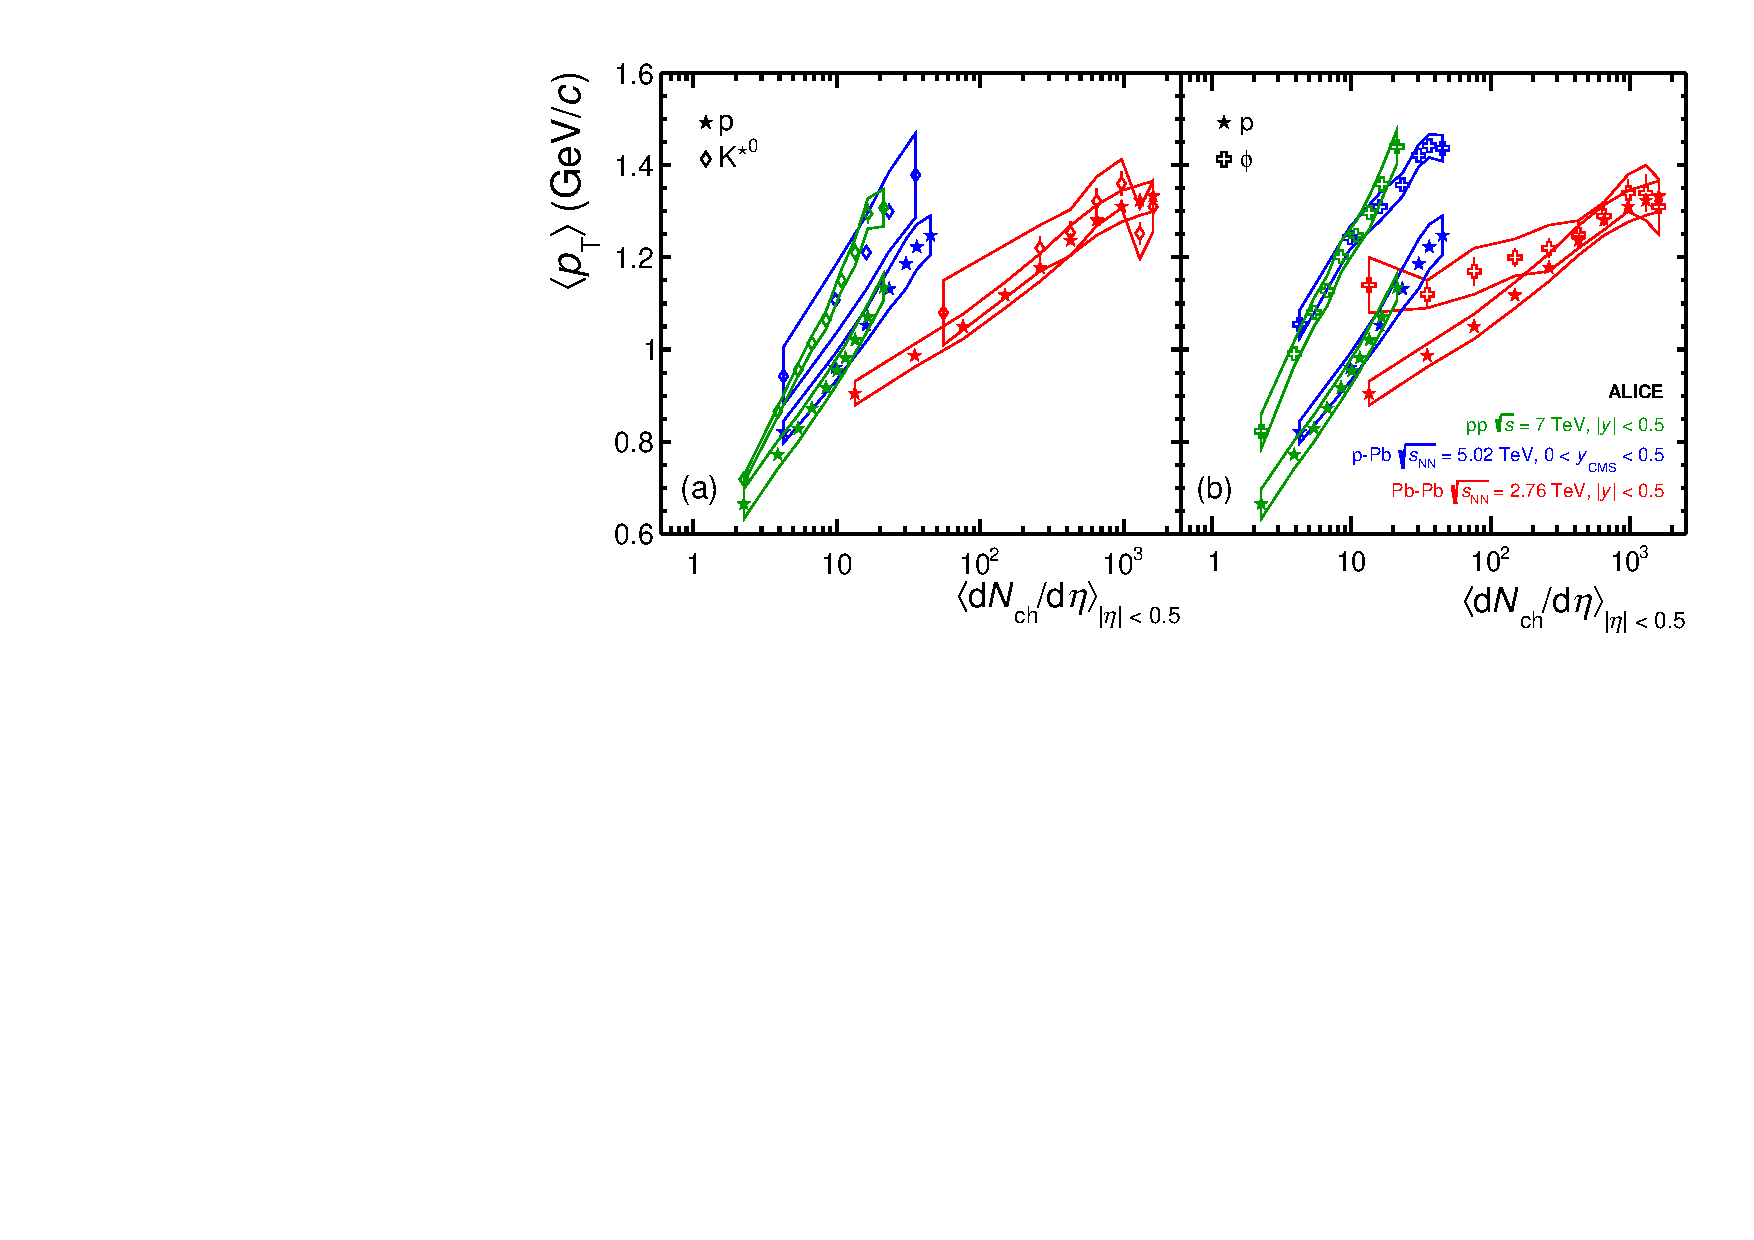
\includegraphics[width=0.865\textwidth]{figures/LongPaper_meanPtVsSystemSize.pdf}}
    \end{flushleft}
    \caption{Average transverse momentum (a) \kstar\ (left) and (b) $\phi$ compared to protons as a function of 
    charged-particle multiplicity density.} 
    \label{fig:MeanPtResonancesVsProton}
\end{figure*}  

The multiplicity dependence of identified particle yields relative to pions is compared 
to \pPb\ and \PbPb\ results in Fig.~\ref{fig:dNdyRatios}. Particles with a larger strangeness content are observed
to be produced more abundantly with multiplicity, as can be seen in the $\Lambda/\pi$, $\Xi/\pi$ and $\Omega/\pi$ 
ratios~\cite{Adam:2016emw}. The \p/$\pi$ ratio is observed to be constant within uncertainties
 except for the lowest multiplicity event class. This indicates 
that the increase of hyperon production with respect to pions is a phenomenon that does not originate 
from mass differences but is connected to strangeness content. Furthermore, the relative production of the $\phi$ increases with \dNdeta\ by approximately 20\%, similarly to the
\lmb, a single-strange baryon. This suggests that $\phi$ production cannot be
described solely by considering net strangeness or number of strange quark constituents. The
\kstar/$\pi$ ratio, on the other hand, exhibits a hint of a decrease with multiplicity. In nuclear collisions, 
this decrease is more pronounced and is typically considered a consequence of the rescattering of 
\kstar\ decay daughters during a hadronic phase of the system evolution \cite{Abelev:2014uua,Bleicher:2003ij,Markert:2002rw}. 
All these observations are consistent with previous measurements in \pPb~\cite{Abelev:2013haa,Adam:2015vsf,Adam:2016bpr} and indicate that relative particle abundances can be described as a universal function of charged-particle density in 
pp and \pPb\ collisions. 

\begin{figure*}[t!]
  \begin{flushleft}
    \center{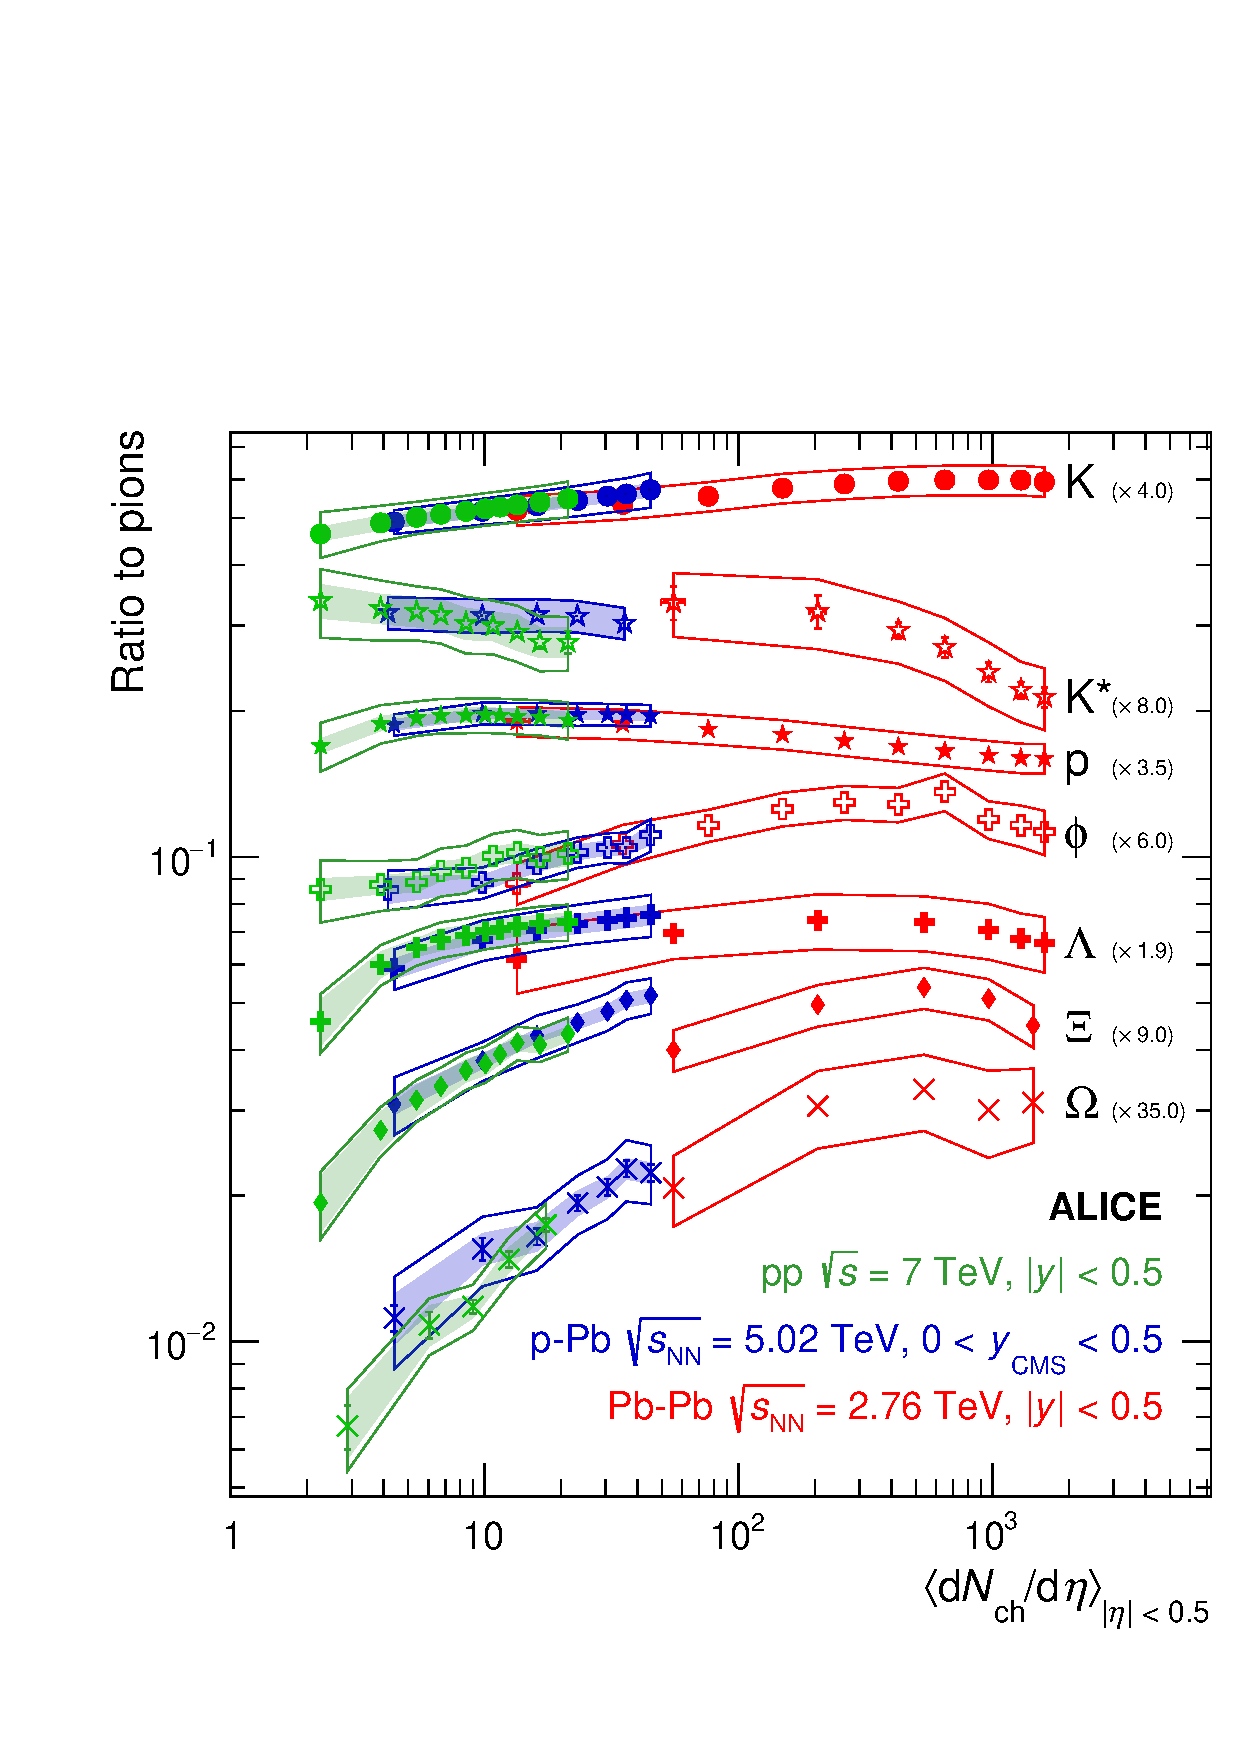
\includegraphics[width=0.675\textwidth]{figures/Results_dNdyRatioVersusV0M_AllSystems.pdf}}
    \end{flushleft}
    \caption{Integrated particle-to-pion ratios as a function of \avdNdeta\ for pp, p-Pb and Pb-Pb collisions. Reference p-Pb and Pb-Pb data from \cite{Abelev:2013haa, Adam:2015vsf, 2016720, Abelev:2013xaa,2014196}.}
    \label{fig:dNdyRatios}
\end{figure*}  


